\lhead{\emph{Preliminary}}
\chapter{Preliminary}
The purpose of this section is to provide an introduction to the concepts and background of our research. By doing so, we hope to provide readers with a better understanding of the context in which our work is situated, and make it easier for them to grasp the key ideas and contributions of our research.

To achieve this goal, we provide an overview of the field of learned indexes and its relevance to data access and manipulation operations and the model used in Learned Index.

In addition, we provide background information on the \acrshort{lipp} approach, which is the foundation of our research. We discuss the structure of \acrshort{lipp}'s node-based index and the components that make it work, such as the gapped array, bitmap index, and linear regression model. We also highlight some of the key features and benefits of \acrshort{lipp}, as well as its limitations.

\section{Linear Regression}
Linear regression is a widely used statistical technique for modeling the relationship between two variables, namely the independent variable, denoted as x, and the dependent variable, denoted as y. The objective of linear regression is to find the best fitting line that represents the relationship between the two variables in the most accurate way possible. The line is represented by the equation $y = mx + c$, where $m$ represents the slope of the line, and $c$ represents the y-intercept.

The main purpose of linear regression is to make predictions based on the relationship between the two variables. In the case of a machine-learned index, linear regression is used to predict the location of the keys in the gapped array. This is done by training a model on a dataset of key and its position. The model learns the relationship between the keys and its location, and can then be used to predict the key's location for new queries.

The process of finding the best fitting line involves minimizing the sum of the squared differences between the actual y-values and the predicted y-values for each data point. This method is known as the method of least squares, and it ensures that the line fits the data points as closely as possible.

One of the reasons why linear regression is used in machine-learned indexes is its simplicity and interpretability. The linear regression model can be easily understood and implemented, and the output can be used to build an index that can efficiently look up rows in the table. Moreover, linear regression can handle large datasets, making it an ideal choice for machine-learned indexes.

In contrast, neural network models can be more complex and computationally expensive, which may cause a large overhead in operations \cite{CasedLearnedIndex}. Therefore, linear regression is a more efficient and practical choice for machine-learned indexes. However, the choice of machine learning algorithm depends on the specific requirements and characteristics of the dataset.

\section{Model-Based Insertion}
\begin{figure}
    \centering
    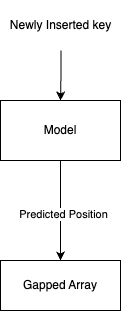
\includegraphics[width=25mm,scale=0.5]{Figures/ModelBasedInsert.png}
    \caption{
     Model-Based Insertion
    }
    \label{fig:model-basedinsertion}
\end{figure}
Model-Based Insertion is essentially an insertion strategy that uses the learned model to determine where newly inserted keys should be placed in the gapped array, previously mentioned in previous section as an array that reserved spaces in between the keys for new insertion, that constitutes the learned index. The algorithm uses the model to predict the location of the new key, and then places it accordingly to ensure that the learned index can efficiently support insert operations. This is achieved by mapping the keys to the linear regression slope of the model, ensuring that the newly inserted keys fit seamlessly within the existing index structure (Figure \ref{fig:model-basedinsertion}).


\acrfull{lipp} adopts a different approach to handling insertion operations compared to other learned indexes such as \acrshort{alex} and PGM \cite{PGM}. Rather than shifting elements or storing them in a temporary buffer to merge later, \acrshort{lipp} employs node creation. This technique involves creating a new node for each new key that is inserted into the index. By creating a new node for each key, \acrshort{lipp} is able to optimize the search operation by ensuring that the output position from the model is exact and precise. This means that \acrshort{lipp} does not need to perform extra searches to locate the key.

However, while \acrshort{lipp}'s node creation approach has several benefits, it also has some limitations. One of the primary concerns with this approach is that it could result in the tree height growing, which could negatively impact the performance of the index. The height of the tree is a critical factor in determining the time complexity of the search operation, and an increase in the height of the tree could result in search operations becoming bound to the height of the tree.
\section{Learned Index Precise Position} \label{LIPP}
\begin{figure}
    \centering
    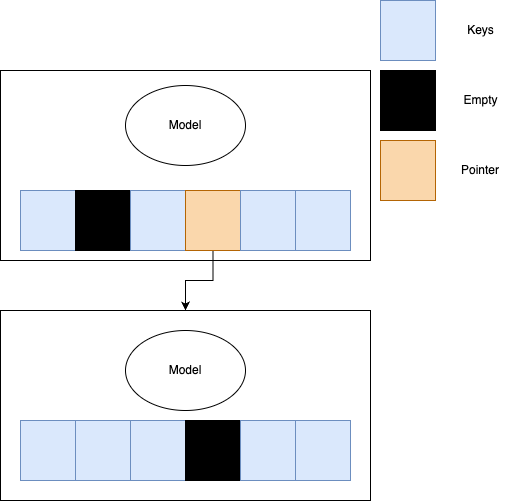
\includegraphics[width=100mm,scale=1]{Figures/LippNode.png}
    \caption{
     \acrshort{lipp} node structure
    }
    \label{fig:lipp-node}
\end{figure}
\acrshort{lipp} achieves prediction precision by using a node-based structure that includes a gapped array, a bitmap index, and a linear regression model (Figure \ref{fig:lipp-node}). These components work together to enable accurate and efficient key access.

Furthermore, \acrshort{lipp} introduces the adjustments or branch pruning to reduce the height of the tree. The conditions to trigger the adjustments are (1) current depth after previous adjustments should not be more than $\beta$ times (set to 2 by default) the previous adjustment, and (2) \conflict number should not exceed $\alpha$ (set to 0.1 by default) from the previous adjustments \cite{LIPP}. 

In this research, we aim to build on the foundations of \acrshort{lipp} by developing an algorithm that further enhances its performance. Our algorithm will focus on optimizing performance of \acrshort{lipp}, specifically by improving the gap placement strategy. By doing so, we aim to improve the accuracy and efficiency of key access operations, enabling faster and more reliable data access and manipulation.
